
\documentclass[letterpaper, 10 pt, conference]{ieeeconf}  % Comment this line out if you need a paper

%\documentclass[a4paper, 10pt, conference]{ieeeconf}      % Use this line for a4 paper

\IEEEoverridecommandlockouts

\overrideIEEEmargins                                      % Needed to meet printer requirements.

% See the \addtolength command later in the file to balance the column lengths
% on the last page of the document
\usepackage{cite}
% The following packages can be found on http:\\www.ctan.org
\usepackage{graphicx} % for pdf, bitmapped graphics files
%\usepackage{epsfig} % for postscript graphics files
%\usepackage{mathptmx} % assumes new font selection scheme installed
%\usepackage{times} % assumes new font selection scheme installed
\usepackage{amsmath} % assumes amsmath package installed
\usepackage{amssymb}  % assumes amsmath package installed
\usepackage{math}
\usepackage{aircraftshapes}
\usepackage[caption=false]{subfig} % subfigures.  false option prevents conflicts in caption styling with other packages
%\usepackage{natbib}
%\usepackage{standalone}
\usepackage{tikz}
\usetikzlibrary{positioning}
\usetikzlibrary{shapes,arrows}
\tikzstyle{pre}=[<-,>=stealth,thick]
\tikzstyle{post}=[->,>=stealth,thick]
\tikzstyle{prepost}=[<->,>=stealth,thick]
\usetikzlibrary{automata,positioning,graphs,calc}

\usepackage{graphicx}
\usepackage{color}
\usepackage{pgfplots}
\pgfplotsset{compat=1.15}
\usepackage{pgf-umlsd}
\usepackage{ifthen}
\usepackage{graphicx}
\usepackage{hyperref}
\usepackage{cleveref}


\usepackage[ruled,longend,linesnumbered]{algorithm2e}
%
%\RequirePackage{fix-cm}

\usepackage{pgfplots}
% \usepackage{fancyhdr}
% \pagesty

\usepackage{xcolor}
\newcommand{\todo}[1]{{\color{blue}[TODO: #1]}}
\newcommand{\response}[1]{{\color{green}[RESPONSE: #1]}}

\title{\LARGE \bf
	Evolutionary Nonlinear Model Predictive Control \\ on a Fixed-Wing and Multirotor
}

%\titlerunning{Short form of title}        % if too long for running head

\author{Jaron Ellingson$^{1}$, Mathew Haskell$^{2}$%
	%	\thanks{*This material is based upon work supported by the National Science Foundation under Grant No. 1727010. This work is also supported by the Center for Unmanned Aircraft Systems (C-UAS), a National Science Foundation Industry/University Cooperative Research Center (I/UCRC) under NSF award No. IIP-1161036 along with significant contributions from C-UAS industry members.}% <-this % stops a space
	\thanks{$^{1}$ Jaron Ellingson is an MS candidate in the Department of Mechanical Engineering, Brigham Young University
		{\tt\small jaronce@byu.edu}}%
	\thanks{$^{2}$ Mathew Haskell is a PhD candidate in the Department of Mechanical Engineering, Brigham Young University
		{\tt\small mathew.haskell@byu.edu}}%
}

\begin{document}
	\maketitle
	\thispagestyle{empty}
	\pagestyle{empty}
	
	\date{Received: date / Accepted: date}
	% The correct dates will be entered by the editor
	
	
	\maketitle
	
	\begin{abstract}
		Real-time model predictive control (MPC) is limited to short time horizons and linear systems because the optimization complexity is too large with long time horizons and nonlinear systems. For this reason, MPC is typically accomplished using linearized models and convex optimization solvers. We seek to explore evolutionary algorithms allowing for nonlinear models and constraints, non-convex costs, and extended time horizons.
		
		Our contributions include extending nonlinear evolutionary MPC to flight vehicles, fixed-wing and multirotor UAVs, as well as enhancing the evolutionary algorithm. We also intend to parameterize the design space of the optimization to reduce solve times. These contributions validate the robust and effective nature of the algorithm.
		
		% \PACS{PACS code1 \and PACS code2 \and more}
		% \subclass{MSC code1 \and MSC code2 \and more}
	\end{abstract}
	
	%\section{Project Direction}
	
	
	%Real-time model predictive control (MPC) is limited to short time horizons and linear systems because the optimization complexity is too large with long time horizons and nonlinear systems. For this reason, MPC is typically accomplished using linearized models and convex optimization solvers. We seek to explore evolutionary algorithms allowing for nonlinear models and constraints, non-convex costs, and extended time horizons. 
	
	%This work is a continuation of the work accomplished in \cite{hyatt2020parameterized} which is developed to parameterize long time horizons. Our contributions include extending nonlinear evolutionary MPC to flight vehicles, fixed-wing and multirotor UAVs, as well as enhancing the evolutionary algorithm. We also intend to parameterize the design space of the optimization to reduce solve times. These contributions will validate the robust and effective nature of the algorithm.
	
	%While parallelization of the evolutionary algorithm allows for real-time control, writing the code to parallelize the algorithm might be out of the scope for this project. A neural network is used in the NEMPC algorithm in \cite{hyatt2019real}, which interfaced with the GPU under the hood. This work seeks to implement NEMPC without using a neural network, making parallelization more difficult.
	
	
	\section{Introduction}
	
	In \cite{hyatt2017real}, linear MPC was performed in real-time on a robotic arm using an evolutionary optimization algorithm rather than a typical convex solver. To make the algorithm real-time, each state propagation in the evolutionary algorithm during a single generation occurred in parallel on a graphics processing unit (GPU). GPU's are known to be fast at matrix multiplications, which the linearized model provided.
	
	The previous work using an evolutionary algorithm was continued in \cite{hyatt2019real} where nonlinear dynamics were used as the model for real-time MPC. The key change in this work from \cite{hyatt2017real} is that the nonlinear dynamics were approximated using a neural network. The neural network was able to learn the nonlinear dynamics in a way that still utilized matrix multiplications, allowing for parallelization of the genetic algorithm on a GPU.
	
	In \cite{hyatt2020parameterized}, the evolutionary MPC algorithm is compared to a MPC using a QP solver both with a parameterized optimization design space to reduce the number of design variables. Both algorithms are capable of real-time control of nonlinear robotic arms. With MPC, the optimization design variable is the future trajectory of control inputs that should be applied to the system over a finite time horizon. This work used a piece-wise linear function to parameterize the trajectory of future inputs, usually with only 2 lines (3 points). This allowed for a significant reduction in the search space of the optimization and thus, faster solve times. With the parameterization, the solve times of both algorithms are capable of running control at over 100 Hz. MPC using the QP solver was still faster than the parallelized NEMPC, but the evolutionary algorithm allows for a nonlinear model.
	
	\section{Model Predictive Control}
	
	
	The MPC problem is formulated by
	
	\begin{equation}
	\label{eq:objective}
	\begin{aligned}
	\text{minimizing} & \quad J= \sum_{k=0}^{T-1} (f(\mathbf{x}_k,\mathbf{u}_k)-\mathbf{x}_{d})^{\top} Q (f(\mathbf{x}_k,\mathbf{u}_k)-\mathbf{x}_{d}) \\
	\text{with respect to} & \quad \mathbf{u}_k  \\
	\text{subject to} & \quad \mathbf{L}_b \le \mathbf{u}_k \le \mathbf{U}_b, \\
	\end{aligned}
	\end{equation}
	
	
	where $f(\mathbf{x}_k,\mathbf{u}_k)$ represents the nonlinear dynamics of either the quadrotor or fixed-wing aircraft applied with Runge-Kutta 4th order approximation. $\mathbf{x}_k$ and $\mathbf{x}_{d}$ are our calculated state and desired state, $\mathbf{u}_k$ represents our inputs, $\mathbf{L}_b$ and $\mathbf{U}_b$ are our lower and upper bounds on the inputs, and $Q$ is a positive semi-definite diagonal matrix which weights the cost of error associated with each state. In \cref{subsub:quad,subsub:fw} we will highlight the differences between the quadrotor and fixed-wing states, desired state, inputs, and cost matrix.
	
	MCP optimizes over a finite time window or horizon to predict what would be an optimal control trajectory. The first control input from the optimal trajectory is applied for one time step and then resolved at the next time step. This pattern continues, essentially predicting future states and then comparing these states to desired states. Usually this problem is solved using linearized models and is solved efficiently with quadratic programming techniques. This linearized problem works well and is popular with nonlinear systems that behave linearly. MPC even works well for a quadrotor \cite{bangura2014real} and a fixed-wing \cite{stastny2017nonlinear}. This project explores using the complete nonlinear dynamic equations for solving the optimization for highly nonlinear systems like a quadrotor and fixed-wing aircraft. We believe that using the full nonlinear dynamics will allow the vehicles to fly more aggressively and efficiently compared to using only the linearized dynamics. 
	
	% So the linearized version also works well for a quadrotor. We might want to re-phrase the last 2 sentences. 
	
	% OK
	
	
	\section{Evolutionary Algorithm}
	
	Most of the work which has been accomplished on our evolutionary algorithm developement was inspired by or implemented from \cite{martins2017multidisciplinary}.
	
	\subsection{Initialization}
	
	To initialize our first population, we choose to implement a Latin-Hypercube sampling algorithm to optimize starting coverage of the design space and allow for input saturation to be enforced. We also decided to insert 1 sample at equilibrium because we know that optimal solutions often lay near equilibrium, especially at level or minimal movement flight.
	
	Since it is likely that the current optimal command trajectory will be close to the optimum solved for at the previous time step, the population from the previous solve is used to initialize the population for the current solve. This is a way to warm start the optimization after the first solve. After the warm start feature is active, only 1 generation needs to be used because the population is already close to the optimum. Only running 1 generation of the evolutionary algorithm significantly decreases the solve time to facilitate real-time control.
	
	
	%To help control the aircraft in real time, we decided to implement a warm start mechanism into our algorithm. This warm start was designed to allow the algorithm to first solve for near optimal solution and then use this solution to adjust the inputs according to the current trajectory of the vehicle. For example, we would run the evolutionary algorithm for 200 generations initially, taking roughly 2 seconds to solve. We then take that control action, take a step in the simulation, and then preform the evolutionary algorithm again but for one generation. All subsequent steps perform one generation step but with the last control step's values. We essentially assume that the control has a rough idea of the correct control but the algorithm converges overtime.
	
	
	% -LHS for initial population generation
	
	% -Also add in 1 sample for equilibrium
	
	% -Lot of time can be spent at equilibrium
	
	% -Finds this solution immediately
	
	% -Can add slew rate \todo{I thought we had this but didn't really keep it.}
	
	% -Enforce saturation (bound constraints)
	
	
	\subsection{Fitness}
	
	The cost function in Eq. \eqref{eq:objective} was used to evaluate the fitness of each member of the population, where the dynamics for a quadrotor and a fixed-wing are used for $f(\mathbf{x}_k,\mathbf{u}_k)$. Each input trajectory in the population is independent of the others, meaning that propagating a single generation can be computed in parallel. In this work, we did not parallelize generation propagation; however, our framework will allow for this feature to be added in the future.
	
	% -RK4 integration of dynamics for f(x,u)
	% -Q is positive semi-definite diagonal matrix
	% -Design variables are only $u_k$ vectors
	% -Large reduction of order
	% -Dim = m*N rather than (m+n)*n
	% -With N = 10 and m = 4 gives 40 design variables
	
	
	\subsection{Selection}
	
	For the selection process of the evolutionary algorithm, two methods were implemented for comparison. The first method kept a percentage of the most fit members of the population from generation to generation while introducing a certain number of strangers to form the mating pool. This yields a small mating pool were each member was paired enough times to fill up the population size. The second method was tournament style where each member of the population was randomly paired. The most fit of the pairs formed the first half of the mating pool and the process was repeated to form the second half. This created a mating pool of the same size as the population and the most fit member always appears twice in the pool while the least fit is eliminated. Both of these methods worked, but the tournament style ran faster and was more consistent while the first method had times where it didn't work as well.
	
	% Members from this pool were randomly paired to mate without checking if a certain individual was previously paired. Crossover for these pairs happend by 
	
	% This prevented stagnation and randomly selected two from the top to mate 
	
	
	\subsection{Crossover}
	Two methods were implemented and compared for the crossover portion of the genetic algorithm. One involved creating a child by randomly choosing gene by gene with equal likelihood which parent the gene came from. This provided much variation mixing the parents. The other method was a linear crossover where two children were created as the following points:
	
	\begin{equation}
	\label{eq:child1}
	\begin{aligned}
	\mathbf{x}_{c1}&=0.5\mathbf{x}_{p1}+0.5\mathbf{x}_{pf}, \\
	\mathbf{x}_{c1}&=2\mathbf{x}_{p1}-1\mathbf{x}_{pf},
	\end{aligned}
	\end{equation}
	
	where $\mathbf{x}_{p1}$ is the more fit parent. The first child is the average of the two parents and the second child extrapolates in the direction of the parent with a lower cost. A couple of the best parents were also randomly inserted after the crossover step to ensure that the lowest cost in the population doesn't go up between generations. Both of the methods above function and provide diversity for the next generation. The simulation data in later sections used the linear crossover method because the code executed faster.
	
	
	\subsection{Mutation}
	
	For all mutations, a small amount of Gaussian noise was added. We tried both mutating entire members of the population and mutating each individual gene of each member of the population individually, each method occurring with low probability. It didn't seem to make a difference which of these two methods were used during the mutation phase.
	
	
	
	
	\section{Quadrotor}
	\label{subsub:quad}
	
	This section covers the dynamics and control formulation used for a quadrotor. For this work, inertia was ignored by setting the inputs of the system to be angular velocities rather than torques and assuming the commanded angular velocities are achieved instantaneously. This is a similar assumption made in successive loop closure methods for PID controllers. The state $\mathbf{x}$ and input $\mathbf{u}$ are defined as
	
	\begin{equation}
	\label{eq:quad_xu}
	\mathbf{x}=\begin{bmatrix}\mathbf{p} \\ \boldsymbol{\Theta} \\ \mathbf{v} \end{bmatrix} \text{and}\ \mathbf{u}=\begin{bmatrix}$s$ \\ \boldsymbol{\omega} \end{bmatrix}
	\end{equation}
	
	where, $\mathbf{p}$ is the position of the vehicle in an inertial frame of reference, $\boldsymbol{\Theta}$ represents Euler angles describing the attitude of the vehicle, $\mathbf{v}$ is the velocity of the vehicle in it's own body frame of reference, $s$ is the commanded throttle signal, and $\boldsymbol{\omega}$ is the commanded angular velocities in the body's frame of reference. The state derivative equations are shown in Eqs. \ref{eq:lqr_pdot_true}, \ref{eq:lqr_vdot_true}, and with \ref{eq:lqr_qdot_true} being substituted for Euler angle kinematics. The force term in Eq. \ref{eq:lqr_vdot_true} contains forces from the combined thrust of the propellers, gravity, and a linear drag term:
	
	\begin{equation}
	\label{eq:quad_forces}
	\frac{1}{m}\mathbf{f}^b=-g\frac{s}{s_e}\hat{\mathbf{e}}+gR_I^b\hat{\mathbf{e}}-c_d\mathbf{v}^b_{b/I}
	\end{equation}
	
	where $g$ is the gravity constant, $s_e$ is the quadrotor's equilibrium throttle signal, $c_d$ is a drag coefficient, and $\hat{\mathbf{e}}$ is a unit vector along the z-axis. The throttle term is a linear approximation of thrust. 
	
	Finally, the cost matrix and bound constraints from Eq. \ref{eq:objective} were set as
	
	\begin{equation}
	\begin{aligned}
	Q &= \text{diagonal}(\begin{bmatrix}
	10,10,100,20.5,20.5,20,9.8,9.8,10
	\end{bmatrix}). \\
	\mathbf{L}_b &= \begin{bmatrix}
	0, -\frac{\pi}{2}, -\frac{\pi}{2}, -\frac{\pi}{2}
	\end{bmatrix}, \\
	\mathbf{L}_b &= \begin{bmatrix}
	1, \frac{\pi}{2}, \frac{\pi}{2}, \frac{\pi}{2}
	\end{bmatrix}.
	\end{aligned}
	\end{equation}
	
	The reference command included values for all 3 position states as well as heading and the reference for all other states was set to 0.
	
	
	\section{Fixed-Wing}
	\label{subsub:fw}
	
	The fixed-wing evolutionary and control characteristics are described in this section. We start with the dynamics $f(\mathbf{x}_k,\mathbf{u}_k)$ represents the nonlinear dynamics of a fixed wing aircraft applied with Runge-Kutta 4th order approximation (see Appendix \ref{sec:dynamics} and \cite{beard2012small} for more details). $\mathbf{x}_k$ and $\mathbf{x}_{d}$ are our calculated state and desired state where,
	
	\begin{equation}
	\label{eq:lqr_current_desired_states}
	\mathbf{x}=\begin{bmatrix}\mathbf{p} \\ \mathbf{v} \\ \mathbf{q} \\ \boldsymbol{\omega}\end{bmatrix}.
	\end{equation}
	
	Furthermore, $Q$ is our cost matrix and initialized as,
	
	\begin{equation}
	Q = \text{diagonal}(\begin{bmatrix}
	0,0,100,0,0,0,50,50,50,0,0,0
	\end{bmatrix}).
	\end{equation}
	
	We choose this particular cost because we don't necessarily want the aircraft to hit a particular location but to maintain a desired altitude and heading. 
	
	The desired heading is calculated by the position of the aircraft through a vector field. An example of a vector field can be seen in \Cref{fig:vet_field}. In this figure the aircraft is some distance away from the waypoint path $w_{i-1}$ to $w_i$. \Cref{fig:vet_field} shows the vector field which slowly places the aircraft onto a course to the next waypoint. This vector field allows us to define the commanded heading of the aircraft as we are far away from the desired path. this vector field is defined as,
	
	\begin{equation}
	\check{\chi}=\chi_{l}-\chi_{\infty}\frac{2}{\pi}\tan^{-1}\left(k_{path}\mathbf{e}_{2}\right),
	\end{equation}
	
	where $\chi_l$ is the course angle of our line, and $\check{\chi}$ is the desired course angle. Furthermore, $k_{path}$ is a positive gain and $\chi_\infty$ is the maximum allowed difference between $\check{\chi}$ and $\chi_l$.
	
	We also choose to implement a vector field for maintaining a course on a circular path. The vector field in this case is defined as 
	
	
	\begin{equation}
	\begin{aligned}
	\check{\chi}= & \varphi +  \lambda \left(\frac{2}{\pi}+\tan^{-1}\left(k_{orbit}\frac{d-\rho}{\rho}\right)\right) \\
	\varphi = & atan2\left(p_e-c_e,p_n-c_n\right)+2\pi m,
	\end{aligned}
	\end{equation}
	
	where the orbit angle $\varphi$ needs to wrapped, $\lambda$ determines the direction of the vector field, $p_e$ and $p_n$ and east and north coordinates of the aircraft, $c_e$ and $c_n$ are the coordinates of the circle, $d$ is the distance of the aircraft away from the center of the circle, and $\rho$ is the circle radius (see \cite{beard2012small} for more details on vector fields).
	
	
	\begin{figure}
		\centering
		\begin{tikzpicture}
		\def\length{sqrt(1+(-pi/6*2/pi * atan(0.1*x))^2)}
		\begin{axis}[
		title={},
		domain=-2:2,
		view={0}{90},
		axis background/.style={fill=white},
		xticklabels={},
		yticklabels={},
		ticks=none,
		]
		\addplot3[black,
		quiver={
			u={-pi/6*2/pi * atan(0.1*x)/\length},
			v={1/\length},
			scale arrows=0.3,
		},
		-stealth,samples=15]
		{x};
		\end{axis}
		%\draw [very thick][-latex](160pt,20pt)..controls(100pt,25pt) and (60pt,45pt)..(42pt,58pt);
		%\filldraw(160pt,20pt)circle(2pt) (100pt,25pt)circle (2pt) (60pt,45pt)circle (2pt) (42pt,58pt)circle (2pt);
		\coordinate[label = above:$w_{i}$] (wi) at (97.5pt,161pt);
		\node at (wi)[circle,fill,inner sep=2.5pt]{};
		\coordinate[label = below:$w_{i-1}$] (wi1) at (97.5pt,0pt);
		\node at (wi1)[circle,fill,inner sep=2.5pt]{};
		\draw[very thick] (wi1) -- (wi);
		
		\draw [line width=2pt, dash pattern=on \pgflinewidth off 2pt] plot [smooth, tension=0.75] coordinates {(140pt,37pt) (105pt,60pt) (97.5pt,100pt)};
		\node [aircraft top,fill=black,minimum width=0.75cm,rotate=160] at (150pt,33.5pt) {};
		
		%\filldraw(97.5pt,161pt)circle(2pt) (97.5pt,0pt)circle(2pt);
		%\draw[very thick] (97.5pt,161pt) -- (97.5pt,0pt);
		\end{tikzpicture}
		\caption{A vector field which converges onto a path from one waypoint to another.}
		\label{fig:vet_field}
		
	\end{figure}
	
	
	
	
	Our design variables $\mathbf{u}_k =\begin{bmatrix}s_{a} & s_{e} & s_{t} & s_{r}\end{bmatrix}^{\top}$ represent the control inputs to the system and are constrained to be within certain bounds. The aileron, elevator, and rudder are all constrained to be within $-\pi/2$ to $\pi/2$ radians and the throttle is constrained from 0 to 1. 
	
	%To reduce the number of design variables, I choose to have the inputs applied along a segment of the trajectory and do not choose a new input at every time step. 
	
	%I choose to have 10 control inputs for a time horizon of 1 second with time steps of 0.01 seconds. This means every 0.1 seconds I apply a new control input. \Cref{fig:sub2,fig:cd2} shows only 10 inputs applies over the trajectory of 1 second for two separate test cases.
	
	\begin{figure*}[htbp]
		\centering
		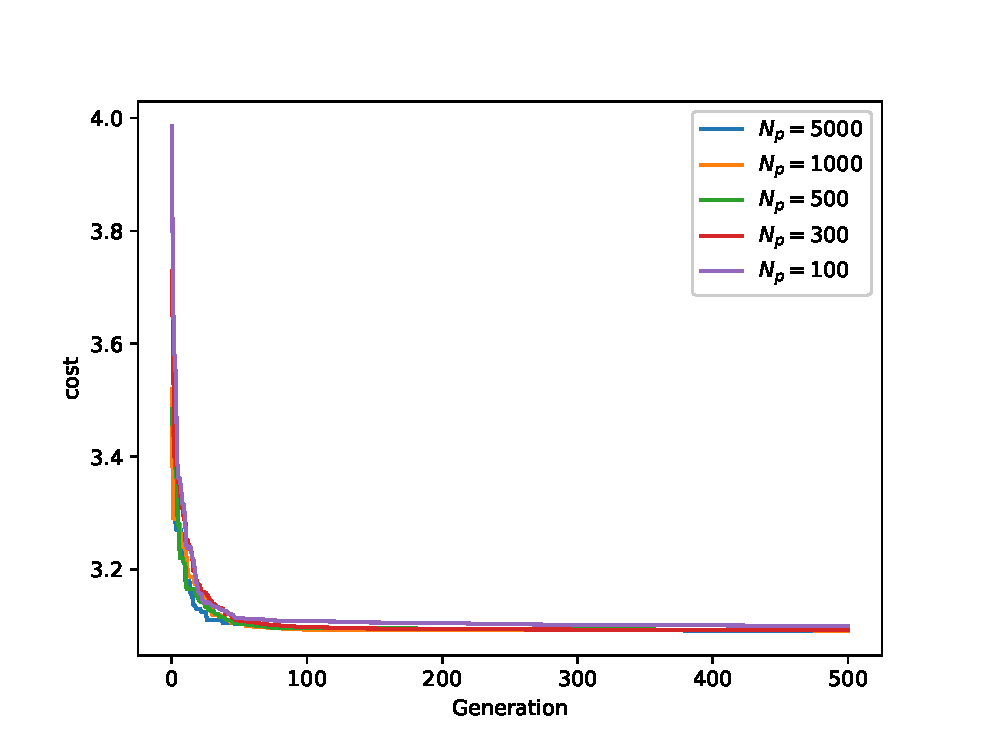
\includegraphics[width=0.45\textwidth]{figures/fixedwing_convergence.eps}
		\caption{Fixed-wing convergence.}
		\label{fig:fw_convergence}
	\end{figure*}
	
	
	We also experimented with the number of generations and population size. \Cref{fig:fw_convergence} highlights convergence for different number of populations. The number of the population appears to matter less with this particular optimization than the number of generations. To allow for our optimization to converge, we choose to run the optimization for 200 generations to start the optimization and then for 1 generation every subsequent MPC solve.
	
	\section{Results}
	
	This section will highlight our results for both vehicles. 
	
	\subsubsection{Quadrotor}
	
	\Cref{fig:quad_convergence} shows the analysis of the quadrotor system to determine an appropriate population size and how many generations should occur in the first MPC solve. After around 200 generations, the cost appears to have converged; however, the small difference in cost from generation 200 to 500 makes a difference. The solution is very close to the actual minimum around generation 200, but the small amount of noise remaining shows up when using the evolutionary algorithm to control the quadrotor. A scenario was simulated where a quadrotor was commanded to move 1 meter East and 1 meter up in altitude from its initial position. This was simulated using a population of both 5000 and 500 where the first MPC solve ran for 200 generations. The simulation results are shown in \Cref{fig:quad_sim5000,fig:quad_sim500}. Using a population size of 5000 provided smoother inputs and outputs with the system compared to the population of 500, which is to be expected. However, both of these simulations generated quite noisy inputs even though they both successfully reached the commanded state. Using the smaller population size allowed the simulation to run in real time, which is a promising sign considering that the algorithm has not yet been parallelized.
	
	\begin{figure*}[htbp]
		\centering
		\includegraphics[width=0.45\textwidth]{figures/quadrotor_convergence.png}
		\caption{Quadrotor convergence.}
		\label{fig:quad_convergence}
	\end{figure*}
	
	\begin{figure*}[htbp]
		\centering
		\subfloat[]{
			\includegraphics[width=0.53\textwidth]{figures/quadrotor_x5000.png}
			\label{fig:quad_positions5000}
		}
		\qquad
		\subfloat[]{
			\includegraphics[width=0.38\textwidth]{figures/quadrotor_u5000.png}
			\label{fig:quad_input5000}
		}
		\caption{Quadrotor simulation using a population size of 5000. Step commands of 1 meter East, 1 meter up in altitude, and 0 for all other states were used as the reference signal. This should theoretically provide the best inputs possible from the evolutionary algorithm after the original 200 generations. \Cref{fig:quad_positions5000} shows the state plots with positions states on the top row, attitude states on the middle row, and velocity states on the bottom row with units of meters and radians accordingly. \Cref{fig:quad_input5000} shows the inputs generated from the NEMPC controller.}
		\label{fig:quad_sim5000}
	\end{figure*}
	
	\begin{figure*}[htbp]
		\centering
		\subfloat[]{
			\includegraphics[width=0.53\textwidth]{figures/quadrotor_x500.png}
			\label{fig:quad_positions500}
		}
		\qquad
		\subfloat[]{
			\includegraphics[width=0.38\textwidth]{figures/quadrotor_u500.png}
			\label{fig:quad_input500}
		}
		\caption{Quadrotor simulation using a population size of 500. Step commands of 1 meter East, 1 meter up in altitude, and 0 for all other states were used as the reference signal. This should provide a realistic notion for the controller's capabilities since this simulation ran in real time. \Cref{fig:quad_positions500} shows the state plots with positions states on the top row, attitude states on the middle row, and velocity states on the bottom row with units of meters and radians accordingly. \Cref{fig:quad_input500} shows the inputs generated from the NEMPC controller.}
		\label{fig:quad_sim500}
	\end{figure*}
	
	\subsubsection{Fixed-Wing}
	
	\Cref{fig:fw_level,fig:fw_offset,fig:fw_circle} show three test cases for the fixed-wing, level flight, merging into level flight, and circular flight. For each case we assumed that the fixed-wing would maintain an altitude of 100 meters and perform the necessary maneuvers to achieve the desired path. 
	
	\begin{figure*}[htbp]
		\centering
		\subfloat[]{
			\includegraphics[width=0.45\textwidth]{figures/fixedwing_positions.eps}
			\label{fig:fw_positions_level}
		}
		\qquad
		\subfloat[]{
			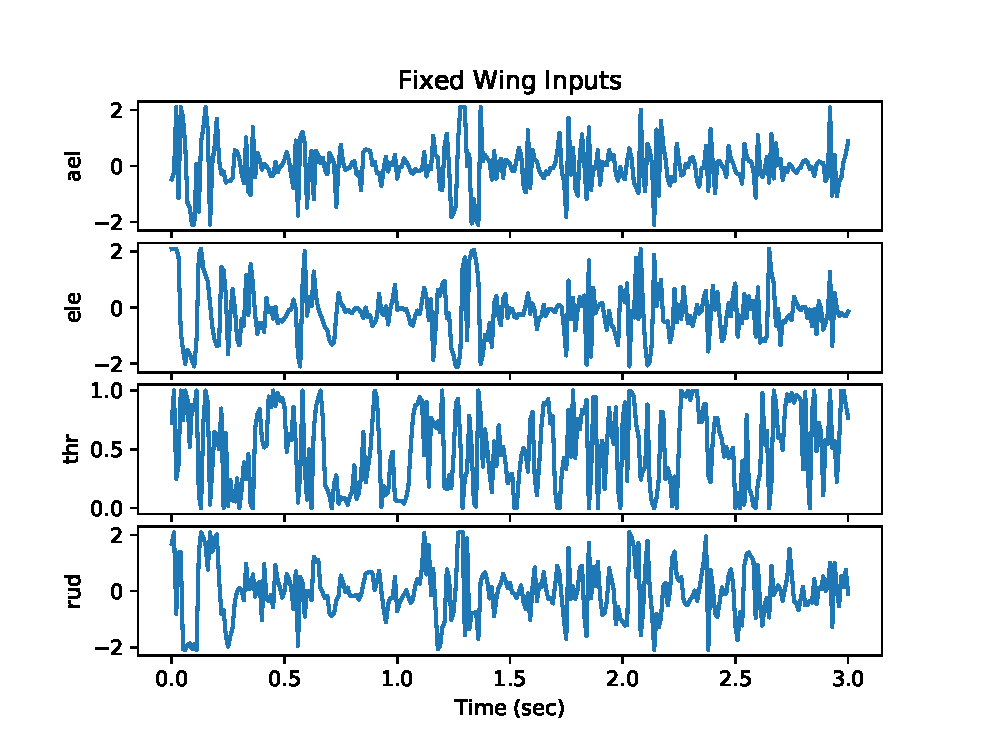
\includegraphics[width=0.45\textwidth]{figures/fixedwing_inputs.eps}
			\label{fig:fw_input_level}
		}
		\caption{Case 1 is the optimization of the aircraft in level flight. The aircraft started at the point (0,0,100) and was commanded to maintain the course on the commanded straight line. It took 37.45 seconds to run 3 seconds of simulation.}
		\label{fig:fw_level}
	\end{figure*}
	
	\begin{figure*}[htbp]
		\centering
		\subfloat[]{
			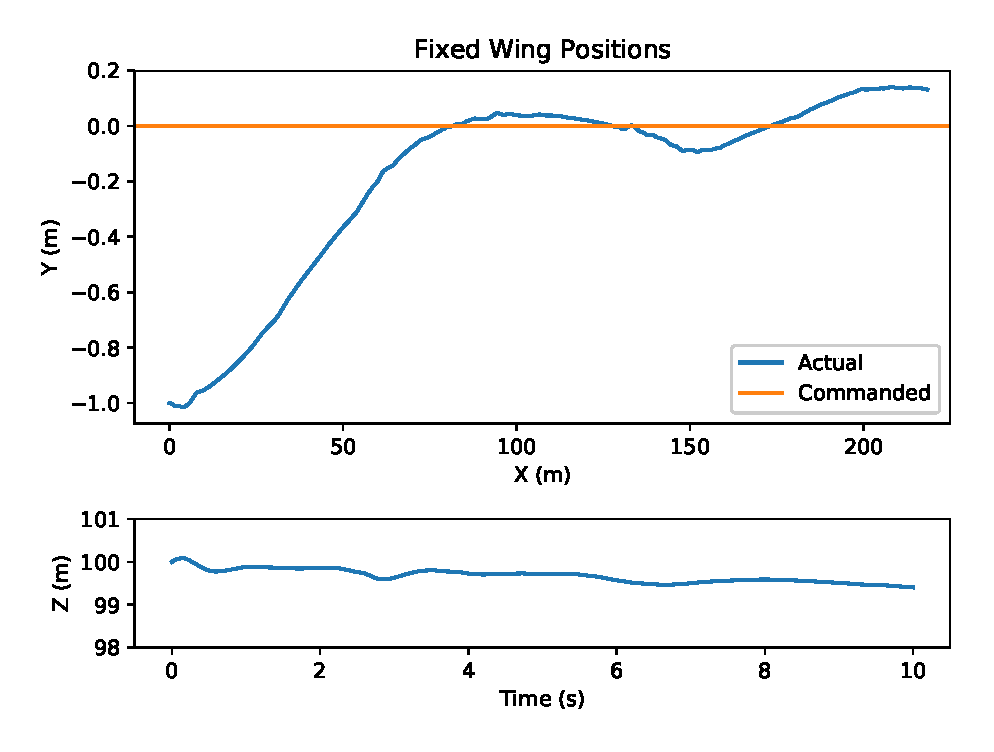
\includegraphics[width=0.45\textwidth]{figures/fixedwing_offset.eps}
			\label{fig:fw_offset_positions}
		}
		\qquad
		\subfloat[]{
			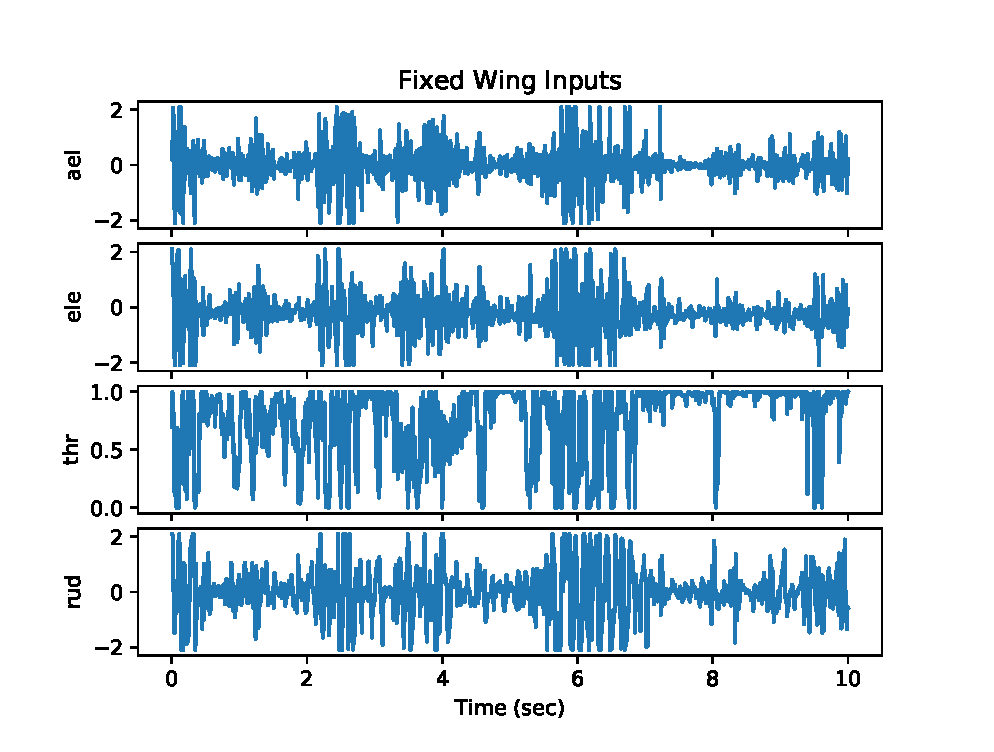
\includegraphics[width=0.45\textwidth]{figures/fixedwing_offset_inputs.eps}
			\label{fig:fw_offset_inputs}
		}
		\caption{Case 2 is the optimization of the aircraft in level flight but with an initial offset starting point. The aircraft started at the point (0,-1,100) and was commanded to maintain the course on the commanded straight line. It took 120.64 seconds to run 10 seconds of simulation.}
		\label{fig:fw_offset}
	\end{figure*}
	
	
	\begin{figure*}[htbp]
		\centering
		\subfloat[]{
			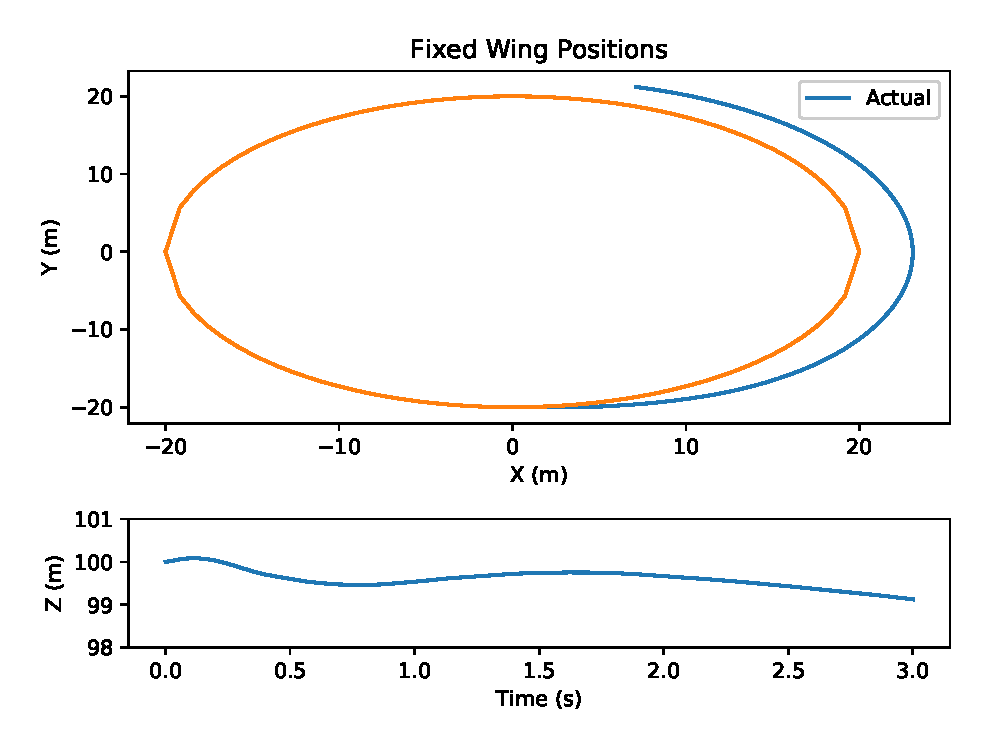
\includegraphics[width=0.45\textwidth]{figures/fixedwing_circle.eps}
			\label{fig:fw_circle_positions}
		}
		\qquad
		\subfloat[]{
			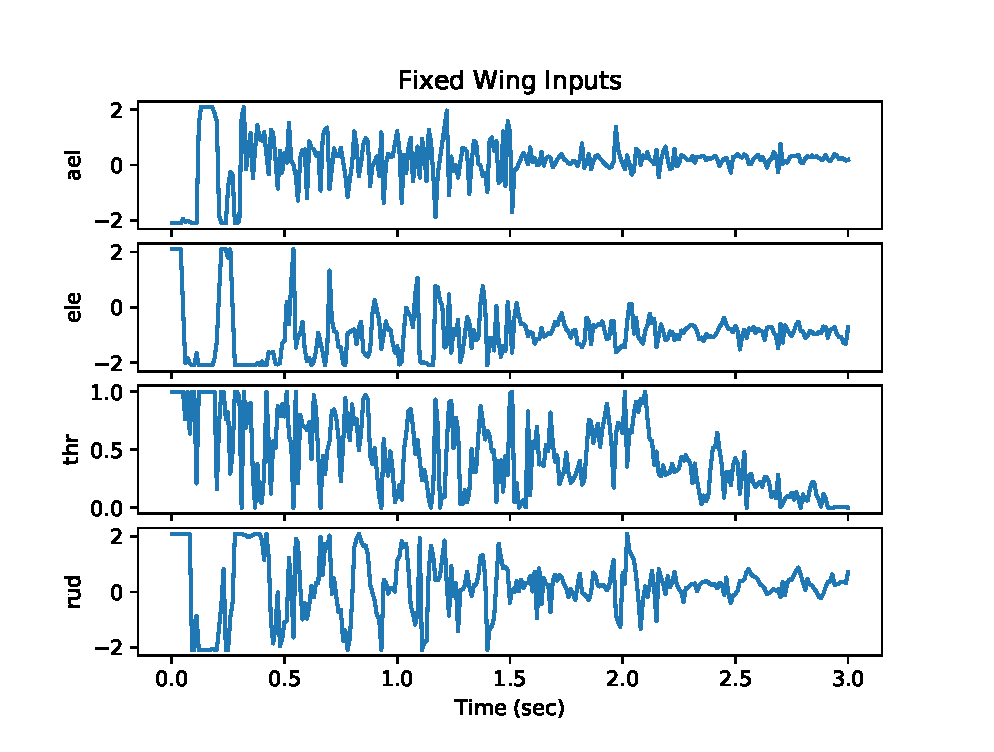
\includegraphics[width=0.45\textwidth]{figures/fixedwing_circle_inputs.eps}
			\label{fig:fw_circle_input}
		}
		\caption{Case 2 is a base case to see if the optimization knows how to keep the aircraft in  flight. It took 37.21 seconds to run 3 seconds of simulation.}
		\label{fig:fw_circle}
	\end{figure*}
	
	\section{Conclusion}
	
	Overall, we consider this a proof of concept for using an evolutionary algorithm for optimizing the control of the UAVs. We are pleased that we were able to control the aircraft in simulation but overall we do not think that the results are better than linear MPC. However, we do think that this is a good starting point for other research and believe that the methods presented can be improved upon.
	
	Future work involves implementing this algorithm on a GPU to speed up the solving time. This might allow for more than one intermediate generation between time steps and result in more accurate and robust solutions. There is also a lot more room to explore all the variety of evolutionary algorithms. Furthermore, we would want to compare with method to other optimal control schemes such as MPC or LQR and compare these schemes on hardware. 
	
	
	\begin{appendices}
		
		\section{Aircraft Dynamics}
		\label{sec:dynamics}
		
		The aircraft's position, velocity, attitude, and angular rate evolve in time according to
		\begin{align}
		\dot{\mathbf{p}}_{b/I}^{I} & =\left(R_{I}^{b}\right)^{\top}\mathbf{v}_{b/I}^{b}\label{eq:lqr_pdot_true}\\
		\dot{\mathbf{v}}_{b/I}^{b} & =\frac{1}{m}\mathbf{f}^{b}-\boldsymbol{\omega}_{b/I}^{b}\times\mathbf{v}_{b/I}^{b}\label{eq:lqr_vdot_true}\\
		\dot{\mathbf{q}}_{I}^{b} & =\boldsymbol{\omega}_{b/I}^{b}\label{eq:lqr_qdot_true}\\
		\dot{\boldsymbol{\omega}}_{b/I}^{b} & =J^{-1}\left(\boldsymbol{\tau}^{b}-\boldsymbol{\omega}_{b/I}^{b}\times J\boldsymbol{\omega}_{b/I}^{b}\right),\label{eq:lqr_omegadot_true}
		\end{align}
		where $m$ is the aircraft's mass, $J$ is the aircraft's inertia matrix, and $\mathbf{f}^b$ and $\boldsymbol{\tau}^b$ are the force and torque applied to the aircraft body~\cite{beard2012small}.
		
		We assume that the aircraft is equipped with the four control inputs: aileron, elevator, throttle, and rudder.
		The aircraft receives a throttle signal $s_t\in\left[0,1\right]$ and signals for aileron, elevator, and rudder given by
		\begin{align}
		s_{a} &= \frac{\delta_{a}}{\delta_{a_{max}}}\in\left[-1,1\right] \\
		s_{e} &= \frac{\delta_{e}}{\delta_{e_{max}}}\in\left[-1,1\right] \\
		s_{r} &= \frac{\delta_{r}}{\delta_{r_{max}}}\in\left[-1,1\right],
		\end{align}
		where $\delta_*$ denotes deflection angle in radians and $\delta_{*_{max}}$ is the physically defined, maximum angle of deflection.
		
		Vehicle air velocity, air speed, angle of attack, and side slip angle are defined by
		\begin{align}
		\mathbf{v}_{a/I}^{b} & =\mathbf{v}_{b/I}^{b}-R_{I}^{b}\mathbf{v}_{w/I}^{I}\\
		V_{a} & =\norm{\mathbf{v}_{a/I}^{b}} \\
		\alpha & =\tan^{-1}\left(\frac{\mathbf{e}_{3}^{\top}\mathbf{v}_{a/I}^{b}}{\mathbf{e}_{1}^{\top}\mathbf{v}_{a/I}^{b}}\right)\\
		\beta & =\sin^{-1}\left(\frac{\mathbf{e}_{2}^{\top}\mathbf{v}_{a/I}^{b}}{V_{a}}\right),
		\end{align}
		where $\mathbf{v}_{w/I}^I$ is the wind velocity expressed in the inertial frame.
		
		Nondimensionalized coefficients of lift and drag are defined by
		\begin{align}
		C_{L}\left(\alpha\right) & =\left(1-\sigma\left(\alpha\right)\right)\left[C_{L_{0}}+C_{L_{\alpha}}\alpha\right]+\sigma\left(\alpha\right) \\ & \quad \left[2\mathrm{sign}\left(\alpha\right)\sin^{2}\alpha\cos\alpha\right]\nonumber\\
		C_{D}\left(\alpha\right) & =C_{D_{p}}+\frac{S\left(C_{L_{0}}+C_{L_{\alpha}}\alpha\right)^{2}}{\pi eb^{2}},
		\end{align}
		where
		\begin{equation}
		\sigma\left(\alpha\right) =\frac{1+e^{-M\left(\alpha-\alpha_{0}\right)}+e^{M\left(\alpha+\alpha_{0}\right)}}{\left(1+e^{-M\left(\alpha-\alpha_{0}\right)}\right)\left(1+e^{M\left(\alpha+\alpha_{0}\right)}\right)}.
		\end{equation}
		Nondimensionalized coefficients of force in the body $x$ and $z$ axes are therefore given by
		\begin{align}
		C_{X}\left(\alpha\right) & =-C_{D}\left(\alpha\right)\cos\alpha+C_{L}\left(\alpha\right)\sin\alpha\\
		C_{X_{q}}\left(\alpha\right) & =-C_{D_{q}}\cos\alpha+C_{L_{q}}\sin\alpha\\
		C_{X_{\delta_{e}}}\left(\alpha\right) & =-C_{D_{\delta_{e}}}\cos\alpha+C_{L_{\delta_{e}}}\sin\alpha\\
		C_{Z}\left(\alpha\right) & =-C_{D}\left(\alpha\right)\sin\alpha-C_{L}\left(\alpha\right)\cos\alpha\\
		C_{Z_{q}}\left(\alpha\right) & =-C_{D_{q}}\sin\alpha-C_{L_{q}}\cos\alpha\\
		C_{Z_{\delta_{e}}}\left(\alpha\right) & =-C_{D_{\delta_{e}}}\sin\alpha-C_{L_{\delta_{e}}}\cos\alpha.
		\end{align}
		
		Consequently, the force and torque expressed in the body frame are given by
		\begin{align}
		\mathbf{f}^{b} & =mR_{I}^{b}\mathbf{g}^{I}+\frac{\rho V_{a}^{2}S}{2}\bigg(C_{F}\left(\alpha,\beta\right)+\left.\frac{1}{2V_{a}}C_{F_{\omega}}\left(\alpha\right)\boldsymbol{\omega}_{b/I}^{b}+ \\ & \quad C_{F_{u}}\left(\alpha\right)\mathbf{u}\right)\bigg)+\rho S_{prop}C_{prop}\mathbf{e}_{3}^{\top}\mathbf{u}\left(V_{a}\\ & \quad+\mathbf{e}_{3}^{\top}\mathbf{u}\left(k_{motor}-V_{a}\right)\right)\cdot\nonumber\left(k_{motor}-V_{a}\right)\mathbf{e}_{1}\nonumber\\
		\boldsymbol{\tau}^{b} & =\frac{\rho V_{a}^{2}S}{2}C_{bc}\bigg(C_{\tau}\left(\alpha,\beta\right)+\frac{1}{2V_{a}}C_{\tau_{\omega}}\boldsymbol{\omega}_{b/I}^{b}+ C_{\tau_{u}}\mathbf{u}\bigg)\\ & \quad-k_{T_{p}}\left(k_{\Omega}\mathbf{e}_{3}^{\top}\mathbf{u}\right)^{2}\mathbf{e}_{1},\nonumber
		\end{align}
		where
		\begin{align}
		\mathbf{u} & =\begin{bmatrix}s_{a} & s_{e} & s_{t} & s_{r}\end{bmatrix}^{\top}\\
		C_{F}\left(\alpha,\beta\right) & =\begin{bmatrix}C_{X}\left(\alpha\right)\\
		C_{Y_{0}}+C_{Y_{\beta}}\beta\\
		C_{Z}\left(\alpha\right)
		\end{bmatrix}\\
		C_{F_{\omega}}\left(\alpha\right) & =\begin{bmatrix}0 & C_{X_{q}}\left(\alpha\right)c & 0\\
		C_{Y_{p}}b & 0 & C_{Y_{r}}b\\
		0 & C_{Z_{q}}\left(\alpha\right)c & 0
		\end{bmatrix}\\
		C_{F_{u}}\left(\alpha\right) & =\begin{bmatrix}0 & C_{X_{\delta_{e}}}\left(\alpha\right)\delta_{e_{max}} & 0 & 0\\
		C_{Y_{\delta_{a}}}\delta_{a_{max}} & 0 & 0 & C_{Y_{\delta_{r}}}\delta_{r_{max}}\\
		0 & C_{Z_{\delta_{e}}}\left(\alpha\right)\delta_{e_{max}} & 0 & 0
		\end{bmatrix}\\
		C_{bc} & =\begin{bmatrix}b & 0 & 0\\
		0 & c & 0\\
		0 & 0 & b
		\end{bmatrix}\\
		C_{\tau}\left(\alpha,\beta\right) & =\begin{bmatrix}C_{l_{0}}+C_{l_{\beta}}\beta\\
		C_{m_{0}}+C_{m_{\alpha}}\alpha\\
		C_{n_{0}}+C_{n_{\beta}}\beta
		\end{bmatrix}\\
		C_{\tau_{\omega}} & =\begin{bmatrix}C_{l_{p}}b & 0 & C_{l_{r}}b\\
		0 & C_{m_{q}}c & 0\\
		C_{n_{p}}b & 0 & C_{n_{r}}b
		\end{bmatrix}\\
		C_{\tau_{u}} & =\begin{bmatrix}C_{l_{\delta_{a}}}\delta_{a_{max}} & 0 & 0 & C_{l_{\delta_{r}}}\delta_{r_{max}}\\
		0 & C_{m_{\delta_{e}}}\delta_{e_{max}} & 0 & 0\\
		C_{n_{\delta_{a}}}\delta_{a_{max}} & 0 & 0 & C_{n_{\delta_{r}}}\delta_{r_{max}}
		\end{bmatrix}.
		\end{align}
		
	\end{appendices}
	
	
	\bibliographystyle{unsrt}
	\bibliography{references} % bibliography data in references.bib
	\bibliographystyle{IEEEtran}
	
\end{document}
